\begin{name}
	{\tenchude}{\tendethi}{LỚP TOÁN THẦY PHÁT}{\thoigian}
\end{name}
\setcounter{ex}{0}\setcounter{bt}{0}
\Opensolutionfile{ans}[ans/ans-2-TT-7-SGD-HoaBinh-23-L1]
%%==========Câu 1

\begin{ex}%[2-TT-7-SGD-Hòa Bình- 2023- Lần 1]%[Nguyễn Cường-EX-6]%[2D1Y1-2]
	Cho hàm số $y=f(x)$ có bảng xét dấu của đạo hàm như sau
	\begin{center}
		
\begin{tikzpicture}
			\tkzTabInit[nocadre=false,lgt=1.2,espcl=2.5,deltacl=0.6]
			{$x$ /0.7,$f'(x)$/0.7}
			{$-\infty$,$-2$, $0$,  $2$, $+\infty$}
			\tkzTabLine{,+,0,-,0,+,0,-,}
		\end{tikzpicture}
	\end{center}
Hàm số đã cho nghịch biến trên khoảng nào dưới đây?
	\choice
	{\True $(-2;0)$}
	{$(-2;2)$}
	{$(0;+\infty)$}
	{$(-\infty;-2)$}
	\loigiai{
		Hàm số nghịch biến trên khoảng $(-2;0)$ do $f'(x)<0$ trên $(-2;0)$.
	}

\end{ex}
%%==========Câu 2
\begin{ex}%[2-TT-7-SGD-Hòa Bình- 2023- Lần 1]%[Nguyễn Cường-EX-6]%[2H3Y1-3]
Trong KG $Oxyz$, cho mặt cầu $(S) \colon x^2+y^2+z^2-4x+2z+4=0$. Tâm $I$ của mặt cầu $(S)$ có tọa độ
	\choice
{\True $I(2;0;-1)$}
{ $I(4;0;-2)$}
{$I(-4;0;2)$ }
{$I(2;0;1)$}
	\loigiai{
		Mặt cầu $(S)$ có tâm $I(2;0;-1)$.
	}
\end{ex}
%%==========Câu 3
\begin{ex}%[2-TT-7-SGD-Hòa Bình- 2023- Lần 1]%[Nguyễn Cường-EX-6]%[2D2Y4-3]
	Hàm số nào sau đây đồng biến trên $\mathbb{R}$?
	\choice
	{$y=\left(\dfrac{1}{3}\right)^x$}
	{$y=\left(\dfrac{\pi}{4}\right)^x$}
	{$y=\left(\dfrac{\sqrt{3}}{2}\right)^x$}
	{\True $y=\left(\dfrac{\mathrm{e}}{2}\right)^x$}
	\loigiai{
		$y=\left(\dfrac{\mathrm{e}}{2}\right)^x$ đồng biến trên $\mathbb{R}$ do cơ số $\dfrac{\mathrm{e}}{2}>1$.
	}
\end{ex}
%%==========Câu 4
\begin{ex}%[2-TT-7-SGD-Hòa Bình- 2023- Lần 1]%[Nguyễn Cường-EX-6]%[2H3Y2-2]
	Trong KG $Oxyz$, cho mặt phẳng $(\alpha)\colon 2x+y-z+1=0$. Véc-tơ nào sau đây \textbf{không} là véc-tơ pháp tuyến của mặt phẳng $(\alpha)$?
	\choice
	{\True $\overrightarrow{n}=(2;1;1)$}
	{$\overrightarrow{n}=(4;2;-2)$}
	{$\overrightarrow{n}=(-2;-1;1)$}
	{$\overrightarrow{n}=(2;1;-1)$}
	\loigiai{
		$\overrightarrow{n}=(2;1;1)$ không là véc-tơ pháp tuyến của mặt phẳng $(\alpha)$.
	}
\end{ex}
%%==========Câu 5
\begin{ex}%[2-TT-7-SGD-Hòa Bình- 2023- Lần 1]%[Nguyễn Cường-EX-6]%[1D3Y3-3]
	Cho cấp số cộng $(u_n)$ có $u_1=3$ và công sai $d=4$. Giá trị của $u_2$ bằng
	\choice
	{$u_2=-1$}
	{$u_2=12$}
	{\True $u_2=7$}
	{$u_2=1$}
	\loigiai{
		Ta có $u_2=u_1+d=3+4=7$.
	}
\end{ex}
%%==========Câu 6
\begin{ex}%[2-TT-7-SGD-Hòa Bình- 2023- Lần 1]%[Nguyễn Cường-EX-6]%[2D4Y1-2]
Trên mặt phẳng tọa độ, điểm biểu diễn của số phức $z=5-3i$ là
	\choice
	{$(-3;5)$}
	{$(5;3)$}
	{$(-5;-3)$}
	{\True $(5;-3)$}
	\loigiai
	{
		Điểm biểu diễn của số phức $z=5-3i$ là $(5;-3)$.
	}
\end{ex}
%%==========Câu 7
\begin{ex}%[2-TT-7-SGD-Hòa Bình- 2023- Lần 1]%[Nguyễn Cường-EX-6]%[2H2Y1-2]
	Cho hình trụ có bán kính đáy là $r=4$ và độ dài đường sinh $\ell =3$. Diện tích xung quanh của hình trụ đã cho bằng
	\choice
	{$12\pi$}
	{\True $24\pi$}
	{$81\pi$}
	{$32\pi$}
	\loigiai{
	Diện tích xung quanh của hình trụ là $S=2\pi r\ell=2\pi\cdot 4\cdot 3=24\pi$.
	}
\end{ex}
%%==========Câu 8
\begin{ex}%[2-TT-7-SGD-Hòa Bình- 2023- Lần 1]%[Nguyễn Cường-EX-6]%[2D4Y1-1]
Phần ảo của số phức $z=1+2i$ là
	\choice
	{$1$}
	{$2i$}
	{$i$}
	{\True $2$}
	\loigiai{
Phần ảo của số phức $z=1+2i$ là $2$.
	}
\end{ex}
%%==========Câu 9
\begin{ex}%[2-TT-7-SGD-Hòa Bình- 2023- Lần 1]%[Nguyễn Cường-EX-6]%[2D2Y3-2]
		Cho $a$, $b$, $c>0$ tùy ý và $a\ne 1$, $c\ne 1$. Mệnh đề nào dưới đây \textbf{sai}?
		\choice
		{$\log_a\left(\dfrac{b}{c}\right)=\log_ab - \log_ac$}
		{$\log_a(bc)=\log_ab+\log_ac$}
		{\True $\log_ab=\dfrac{\log_ca}{\log_cb}$}
		{$\log_ab^n=n\log_ab$}
		\loigiai{
			$\log_ab=\dfrac{\log_ca}{\log_cb}$ là khẳng định sai.
		}
\end{ex}
%%==========Câu 10
\begin{ex}%[2-TT-7-SGD-Hòa Bình- 2023- Lần 1]%[Nguyễn Cường-EX-6]%[2D1Y5-3]
		\immini{
			Cho hàm số $y=f(x)$	có đồ thị như hình vẽ. Phương trình $3f(x)-4=0$ có bao nhiêu nghiệm thực?
			\choice
			{$4$}
			{\True $3$}
			{$2$}
			{$1$}
		}{
		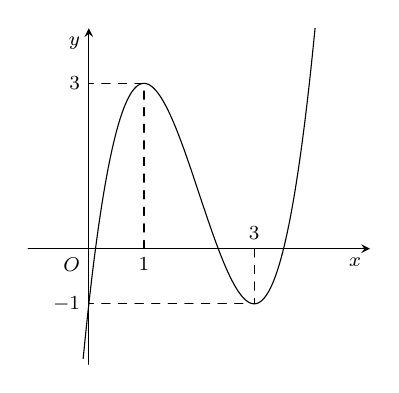
\begin{tikzpicture}[scale=0.7,>=stealth, font=\footnotesize, line join=round, line cap=round]
			\tikzset{every node/.style={scale=0.9}}
			\draw[->] (-1.1,0)--(5.1,0) node[below left] {$x$};
			\draw[->] (0,-2.1)--(0,4) node[below left] {$y$};
			\draw (0,0) node [below left] {$O$};
			\draw[dashed,thin](3,0)--(3,-1)--(0,-1);
			\draw[dashed,thin](1,0)--(1,3)--(0,3);
			\begin{scope}
				\clip (-1,-2) rectangle (5,4);
				\draw[samples=200,domain=-0.25:4.25,smooth,variable=\x] plot (\x,{1*((\x)^3)+-6*((\x)^2)+9*(\x)-1});
			\end{scope}
			\path
			(0,-1)node[left]{$-1$}
			(0,3)node[left]{$3$}
			(1,0)node[below]{$1$}
			(3,0)node[above]{$3$}
			;
		\end{tikzpicture}		
	}
		\loigiai{
			\immini{
	Ta có $3f(x)-4=0\Leftrightarrow f(x)=\dfrac{4}{3}$. Khi đó số nghiệm của phương trình chính là số giao điểm của đồ thị $y=f(x)$ với đường thẳng $y=\dfrac{4}{3}$. Nhìn vào hình vẽ ta thấy có ba giao điểm.\\
	Vậy phương trình đã cho có ba nghiệm.
}{
\begin{tikzpicture}[scale=0.7,>=stealth, font=\footnotesize, line join=round, line cap=round]
	\tikzset{every node/.style={scale=0.9}}
	\draw[->] (-1.1,0)--(4,0) node[below left] {$x$};
	\draw[->] (0,-2.1)--(0,5.1) node[below left] {$y$};
	\draw (0,0) node [below left] {$O$};
	\draw[dashed,thin](3,0)--(3,-1)--(0,-1);
	\draw[dashed,thin](1,0)--(1,3)--(0,3);
	\begin{scope}
		\clip (-1,-2) rectangle (5,4);
		\draw[samples=200,domain=-0.25:4.25,smooth,variable=\x] plot (\x,{1*((\x)^3)+-6*((\x)^2)+9*(\x)-1});
	\end{scope}
	\path
	(0,-1)node[left]{$-1$}
	(0,3)node[left]{$3$}
	(1,0)node[below]{$1$}
	(3,0)node[above]{$3$}
	;
	\draw (-1,1.34)--(4,1.34)node[above left]{$y=\dfrac{4}{3}$};
\end{tikzpicture}
}
		}
	\end{ex}
%%==========Câu 11
\begin{ex}%[2-TT-7-SGD-Hòa Bình- 2023- Lần 1]%[Nguyễn Cường-EX-6]%[2H3Y3-1]
	Trong KG $Oxyz$, cho đường thẳng $d\colon \dfrac{x-2}{-1}=\dfrac{y-1}{2}=\dfrac{z+3}{1}$. Véc-tơ nào dưới đây là một véc-tơ chỉ phương của $d$?
	\choice
	{$\overrightarrow{u}=(1;2;-3)$}
	{$\overrightarrow{u}=(2;1;-3)$}
	{$\overrightarrow{u}=(2;1;1)$}
	{\True $\overrightarrow{u}=(-1;2;1)$}
	\loigiai{
		$\overrightarrow{u}=(-1;2;1)$ là một véc-tơ chỉ phương của $d$.
	}
\end{ex}
%%==========Câu 12
\begin{ex}%[2-TT-7-SGD-Hòa Bình- 2023- Lần 1]%[Nguyễn Cường-EX-6]%[2D1Y3-1]
\immini
{
	Cho hàm đa thức $y=f(x)$ có đồ thị là đường cong như hình bên. Giá trị nhỏ nhất $m$ của hàm số đã cho trên đoạn $[1;3]$ là
		\choice
		{$m=2$}
		{$m=3$}
		{\True $m=-1$}
		{$m=0$}
	}
{
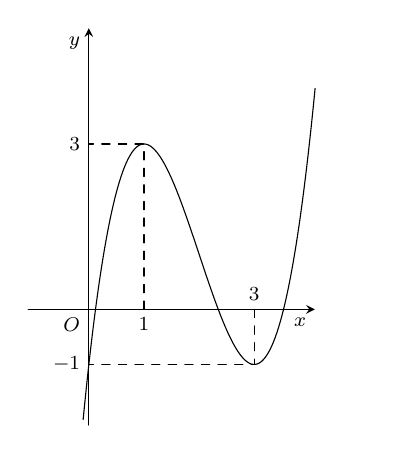
\begin{tikzpicture}[scale=0.7,>=stealth, font=\footnotesize, line join=round, line cap=round]
	\tikzset{every node/.style={scale=0.9}}
	\draw[->] (-1.1,0)--(4.1,0) node[below left] {$x$};
	\draw[->] (0,-2.1)--(0,5.1) node[below left] {$y$};
	\draw (0,0) node [below left] {$O$};
	\draw[dashed,thin](3,0)--(3,-1)--(0,-1);
	\draw[dashed,thin](1,0)--(1,3)--(0,3);
	\begin{scope}
		\clip (-1,-2) rectangle (5,4);
		\draw[samples=200,domain=-0.25:4.25,smooth,variable=\x] plot (\x,{1*((\x)^3)+-6*((\x)^2)+9*(\x)-1});
	\end{scope}
	\path
	(0,-1)node[left]{$-1$}
	(0,3)node[left]{$3$}
	(1,0)node[below]{$1$}
	(3,0)node[above]{$3$}
	;
\end{tikzpicture}
}
		\loigiai{
	 Giá trị nhỏ nhất $m$ của hàm số đã cho trên đoạn $[1;3]$ là $-1$.
		}
\end{ex}
%%==========Câu 13
\begin{ex}%[2-TT-7-SGD-Hòa Bình- 2023- Lần 1]%[Nguyễn Cường-EX-6]%[2H1Y3-2]
	Cho khối lăng trụ có diện tích đáy $B=2a^2$ và chiều cao $h=3a$. Thể tích $V$ của khối lăng trụ đã cho bằng
	\choice
	{\True $V=6a^3$}
	{$V=2a^2$}
	{$V=3a^3$}
	{$V=2a^3$}
	\loigiai{
	Ta có $V=Bh=6a^3$.
	}
\end{ex}
%%==========Câu 14
\begin{ex}%[2-TT-7-SGD-Hòa Bình- 2023- Lần 1]%[Nguyễn Cường-EX-6]%[2D3Y1-1]
	Cho hàm số $f(x)=\sin x+1$. Khẳng định nào dưới đây \textbf{đúng}?
	\choice
	{$\displaystyle\int f(x)\mathrm{\,d}x=\cos x+\dfrac{x^2}{2}+C$}
	{\True $\displaystyle\int f(x)\mathrm{\,d}x=-\cos x+x+C$}
	{$\displaystyle\int f(x)\mathrm{\,d}x=\cos x+x+C$}
	{$\displaystyle\int f(x)\mathrm{\,d}x=-\cos x+\dfrac{x^2}{2}+C$}
	\loigiai{
	$\displaystyle\int \left(\sin x+1\right)\mathrm{\,d}x=-\cos x+x+C$.
	}
\end{ex}
%%==========Câu 15
\begin{ex}%[2-TT-7-SGD-Hòa Bình- 2023- Lần 1]%[Nguyễn Cường-EX-6]%[2H2Y2-1]
	Cho khối cầu $(S)$ có bán kính bằng $3$. Thể tích $V$ của khối cầu đã cho bằng
	\choice
	{$V=9\pi$}
	{$V=108\pi$}
	{$V=27\pi$}
	{\True $V=36\pi$}
	\loigiai{
		Ta có $V=\dfrac{4}{3}\pi R^3=\dfrac{4}{3}\pi\cdot 3^3=36\pi$.
	}
\end{ex}
%%==========Câu 16
\begin{ex}%[2-TT-7-SGD-Hòa Bình- 2023- Lần 1]%[Nguyễn Cường-EX-6]%[2D3Y1-1]
	Cho $\displaystyle\int x^2\mathrm{\,d}x=F(x)+C$. Khẳng định nào dưới đây \textbf{đúng}?
	\choice
	{$F'(x)=\dfrac{x^3}{3}$}
	{$F'(x)=x$}
	{\True $F'(x)=x^2$}
	{$F'(x)=2x$}
	\loigiai{
		Theo định nghĩa nguyên hàm ta có $F'(x)=x^2$.
	}
\end{ex}
%%==========Câu 17
\begin{ex}%[2-TT-7-SGD-Hòa Bình- 2023- Lần 1]%[Nguyễn Cường-EX-6]%[2D1Y2-2]
	Cho hàm số $y=f(x)$ liên tục trên $\mathbb{R}$ và có bảng xét dấu $f'(x)$ như sau
	\begin{center}
		
\begin{tikzpicture}
			\tkzTabInit[nocadre=false,lgt=1.2,espcl=2.5,deltacl=0.6]
			{$x$ /0.7,$f'(x)$/0.7}
			{$-\infty$,$-3$,$2$, $3$, $4$, $+\infty$}
			\tkzTabLine{,-,0,+,0,+,0,-,0,+,}
		\end{tikzpicture}
	\end{center}
Số điểm cực trị của hàm số đã cho là
	\choice
	{\True $3$}
	{$1$}
	{$4$}
	{$2$}
	\loigiai{
		Đạo hàm hàm số đổi dấu qua các điểm $x=-3$; $x=3$ và $x=4$.\\
		Do đó hàm số có $3$ điểm cực trị.
	}
\end{ex}
%%==========Câu 18
\begin{ex}%[2-TT-7-SGD-Hòa Bình- 2023- Lần 1]%[Nguyễn Cường-EX-6]%[2D4Y2-2]
	Cho hai số phức $z_1=1-2i$ và $z_2=2+3i$. Phần thực của số phức $z_1z_2$ bằng
	\choice
	{$-1$}
	{\True $8$}
	{$3$}
	{$-2$}
	\loigiai
	{
		Ta có $z=z_1z_2=(1-2i)(2+3i)=2+3i-4i-6i^2=8-i$.\\
		Phần thực của số phức $z$ là $8$.
	}
\end{ex}
%%==========Câu 19
\begin{ex}%[2-TT-7-SGD-Hòa Bình- 2023- Lần 1]%[Nguyễn Cường-EX-6]%[2D2B6-1]
	Tập nghiệm của bất phương trình $\log_3(4-x)>2$ là
	\choice
	{$(-5;4)$}
	{$(-\infty;4)$}
	{$(-\infty;-5]$}
	{\True $(-\infty;-5)$}
	\loigiai{
		Điều kiện $4-x>0\Leftrightarrow x<4$.\\
		Ta có $\log_3(4-x)>2\Leftrightarrow 4-x> 3^2\Leftrightarrow 4-x>9\Leftrightarrow x<-5$.\\
		Vậy tập nghiệm của bất phương trình là $(-\infty;-5)$.
	}
\end{ex}
%%==========Câu 20
\begin{ex}%[2-TT-7-SGD-Hòa Bình- 2023- Lần 1]%[Nguyễn Cường-EX-6]%[2D3Y2-1]
Nếu $\displaystyle\int\limits_{-3}^2f(x)\mathrm{\,d}x=2$ và $\displaystyle\int\limits_{-3}^2g(x)\mathrm{\,d}x=-5$ thì $\displaystyle\int\limits_{-3}^2\left[f(x)+g(x)\right]\mathrm{\,d}x$ bằng
	\choice
	{$-10$}
	{\True $-3$}
	{$7$}
	{$-2$}
	\loigiai
	{
	Ta có $\displaystyle\int\limits_{-3}^2\left[f(x)+g(x)\right]\mathrm{\,d}x=\displaystyle\int\limits_{-3}^2f(x)\mathrm{\,d}x+\displaystyle\int\limits_{-3}^2g(x)\mathrm{\,d}x=2-5=-3$.
	}
\end{ex}
%%==========Câu 21
\begin{ex}%[2-TT-7-SGD-Hòa Bình- 2023- Lần 1]%[Nguyễn Cường-EX-6]%[2D1Y4-1]
Tiệm cận đứng của đồ thị hàm số $y=\dfrac{x+1}{2+x}$ là đường thẳng có phương trình 
		\choice
		{\True $x=-2$}
		{$y=-2$}
		{$x=2$}
		{$x=1$}
	\loigiai
	{
		Do $\lim\limits_{x\to -2^+}\dfrac{x+1}{2+x}=-\infty$ nên đồ thị hàm số nhận đường thẳng $x=-2$ làm tiệm cận đứng.
	} 
\end{ex}
%%==========Câu 22
\begin{ex}%[2-TT-7-SGD-Hòa Bình- 2023- Lần 1]%[Nguyễn Cường-EX-6]%[2D2Y5-1]
Phương trình $5^x=2$ có nghiệm là
		\choice
		{$x=\dfrac{2}{5}$}
		{$x=\dfrac{5}{2}$}
		{\True $x=\log_52$}
		{$x=\log_25$}
	\loigiai
	{
		Ta có $5^x=2\Leftrightarrow x=\log_52$.
	}
\end{ex}
%%==========Câu 23
\begin{ex}%[2-TT-7-SGD-Hòa Bình- 2023- Lần 1]%[Nguyễn Cường-EX-6]%[2D2Y4-2]
	Trên khoảng $(0;+\infty)$, đạo hàm của hàm số $y=\log_4x$ là
	\choice
	{\True $y'=\dfrac{1}{x\ln 4}$}
	{$y'=-\dfrac{1}{x\ln 4}$}
	{$y'=\dfrac{1}{x}$}
	{$y'=\dfrac{\ln 4}{x}$}
	\loigiai
	{
		Ta có $y'=\dfrac{1}{x\ln 4}$.
	}
\end{ex}
%%==========Câu 24
\begin{ex}%[2-TT-7-SGD-Hòa Bình- 2023- Lần 1]%[Nguyễn Cường-EX-6]%[2D1Y2-2]
	Hàm số $y=f(x)$ có bảng biến thiên như sau
	\begin{center}
		
\begin{tikzpicture}
			\tkzTabInit[nocadre=false,lgt=1.2,espcl=2.5,deltacl=0.6]
			{$x$/0.7,$f’(x)$/0.7,$f(x)$/2}
			{$-\infty$,$-1$,$0$,$1$,$+\infty$}
			\tkzTabLine{ ,-,z,+,z,-,z,+, }
			\tkzTabVar{+/$+\infty$,-/$-4$,+/$3$,-/$-4$,+/$+\infty$}
		\end{tikzpicture}
	\end{center}
Hàm số đã cho đạt cực tiểu tại
		\choice
		{$x=-4$}
		{$x=3$}
		{\True $x=-1$, $x=1$}
		{$x=0$}
	\loigiai
	{
		Hàm số đã cho đạt cực tiểu tại $x=-1$, $x=1$.
	}
\end{ex}
%%==========Câu 25
\begin{ex}%[2-TT-7-SGD-Hòa Bình- 2023- Lần 1]%[Nguyễn Cường-EX-6]%[1D2Y2-1]
Cho tập hợp $X$ có $10$ phần tử. Số tập hợp con gồm $3$ phần tử của $X$ là
	\choice
	{$3!$}
	{$\mathrm{A}_{10}^3$}
	{$\mathrm{A}_{10}^7$}
	{\True $\mathrm{C}_{10}^3$}
	\loigiai{
		Số tập hợp con gồm $3$ phần tử của $X$ là $\mathrm{C}_{10}^3$.
	}
\end{ex}
%%==========Câu 26
\begin{ex}%[2-TT-7-SGD-Hòa Bình- 2023- Lần 1]%[Nguyễn Cường-EX-6]%[2H3B1-3]
	Trong KG $Oxyz$, cho điểm $A(2;-1;-3)$ và $B(0;3;-1)$. Phương trình của mặt cầu đường kính $AB$ là
	\choice
	{$(x+1)^2+(y+1)^2+(z-2)^2=24$}
	{$(x+1)^2+(y+1)^2+(z-2)^2=6$}
	{$(x-1)^2+(y-1)^2+(z+2)^2=24$}
	{\True $(x-1)^2+(y-1)^2+(z+2)^2=6$}
	\loigiai{
		Tâm của mặt cầu đường kính $AB$ là trung điểm $I(1;1;-2)$ của $AB$.\\
		Ta có $\overrightarrow{IA}=(1;-2;-1)$, suy ra $R=IA=\sqrt{1+4+1}=\sqrt{6}$.\\
		Vậy phương trình mặt cầu đường kính $AB$ là $(x-1)^2+(y-1)^2+(z+2)^2=6$.
	}
\end{ex}
%%==========Câu 27
\begin{ex}%[2-TT-7-SGD-Hòa Bình- 2023- Lần 1]%[Nguyễn Cường-EX-6]%[2H3B1-1]
	Trong KG $Oxyz$, tọa độ điểm $M'$ đối xứng với $M(2;-5;4)$ qua mặt phẳng $(Oyz)$ là
	\choice
	{\True $(-2;-5;4)$}
	{$(2;-5;-4)$}
	{$(2;5;4)$}
	{$(2;-5;-4)$}
	\loigiai
	{
Điểm đối xứng với $M(2;-5;4)$ qua mặt phẳng $(Oyz)$ là $M'(-2;-5;4)$.
	}
\end{ex}
%%==========Câu 28
\begin{ex}%[2-TT-7-SGD-Hòa Bình- 2023- Lần 1]%[Nguyễn Cường-EX-6]%[2H3B2-3]
Trong KG $Oxyz$, phương trình mặt phẳng qua ba điểm $A(1;2;-3)$ và song song với mặt phẳng $(Q)\colon 2x-y+3z+2=0$ là
	\choice
	{$2x-y+3z-9=0$}
	{$x+2y-3z-9=0$}
	{$x-2y-3z+9=0$}
	{\True $2x-y+3z+9=0$}
	\loigiai
	{
		Mặt phẳng $(P)\parallel (Q)$ nên $(P)\colon 2x-y+3z+c=0$ với $c\ne 2$.\\
		Do $A(1;2;-3)$ thuộc $(P)$ nên $2-2-9+c=0\Leftrightarrow c=9$.\\
		Vậy $(P)\colon 2x-y+3z+9=0$.
	}
\end{ex}
%%==========Câu 29
\begin{ex}%[2-TT-7-SGD-Hòa Bình- 2023- Lần 1]%[Nguyễn Cường-EX-6]%[2D1B3-1]
	Gọi $M$, $m$ lần lượt là giá trị lớn nhất, giá trị nhỏ nhất của hàm số $y=\dfrac{x+2}{x-1}$ trên đoạn $[2;3]$. Giá trị $M^2+m^2$.
	\choice
	{$\dfrac{25}{4}$}
	{$\dfrac{45}{4}$}
	{\True $\dfrac{89}{4}$}
	{$16$}
	\loigiai
	{
	Ta có $y'=\dfrac{-3}{(x-1)^2}<0$ với mọi $x\in [2;3]$.\\
	Suy ra hàm số nghịch biến trên đoạn $[2;3]$.\\
	Do đó, $m=\min\limits_{[2;3]}y=y(3)=\dfrac{5}{2}$ và $M=\max\limits_{[2;3]}y=y(2)=4$.\\
	Vậy $M^2+m^2=\dfrac{89}{4}$.
	}
\end{ex}
%%==========Câu 30
\begin{ex}%[2-TT-7-SGD-Hòa Bình- 2023- Lần 1]%[Nguyễn Cường-EX-6]%[2D1B1-1]
Hàm số nào dưới đây đồng biến trên khoảng $(-\infty;+\infty)$?
	\choice
	{\True $y=x^3+x$}
	{$y=\dfrac{x+1}{x+3}$}
	{$y=-x^3-3x$}
	{$\dfrac{x-1}{x-2}$}
	\loigiai
	{
	Xét hàm số $y=x^3+x$.\\
	Ta có $y'=3x^2+1>0$ với mọi $x\in \mathbb{R}$.\\
	Do đó hàm số $y=x^3+x$ đồng biến trên $(\infty;+\infty)$.
	}
\end{ex}
%%==========Câu 31
\begin{ex}%[2-TT-7-SGD-Hòa Bình- 2023- Lần 1]%[Nguyễn Cường-EX-6]%[1H3B4-3]
	\immini
	{
	Cho hình chóp $S.ABC$ có đáy là tam giác vuông tại $B$, $AB=a$, $SA$ vuông góc với mặt đáy và $SA=a\sqrt{3}$. Góc giữa mặt phẳng $(SBC)$ và mặt phẳng $(ABC)$
	\choice
	{\True $60^\circ$}
	{$30^\circ$}
	{$90^\circ$}
	{$45^\circ$}
}
{
\begin{tikzpicture}[scale=0.7,>=stealth, font=\footnotesize, line join=round, line cap=round]
	\coordinate (A) at (-2,0);
	\coordinate (B) at (0,-2);
	\coordinate (C) at (3,0);
	\coordinate (S) at ($(A)+(0,4)$);
	\draw(S)--(A) (S)--(B) (S)--(C) (B)--(C) (A)--(B);
	\draw[dashed,thin](A)--(C);
	\pic[draw,thin,angle radius=2mm] {right angle = S--A--B} pic[draw,thin,angle radius=2mm] {right angle = S--A--C};
	\foreach \i/\g in {S/90,A/180,B/-90,C/0}{\draw[fill=white](\i) circle (1.5pt) ($(\i)+(\g:3mm)$) node[scale=1]{$\i$};}
\end{tikzpicture}
}
	\loigiai{
\immini{
Do $BC\perp SA$ và $BC\perp AB$ nên $BC\perp (SAB)$, suy ra $BC\perp SB$.\\
Ta có $\heva{&(SBC)\cap (ABC)=BC\\&BC\perp AB\\&BC\perp SB.}$\\
Suy ra góc giữa mặt phẳng $(SBC)$ và mặt phẳng $(ABC)$ là $\widehat{SBA}$.\\
$\tan\widehat{SBA}=\dfrac{SA}{AB}=\dfrac{a\sqrt{3}}{a}=\sqrt{3}$.\\
Vậy góc giữa mặt phẳng $(SBC)$ và mặt phẳng $(ABC)$ là $\widehat{SBA}=60^\circ$.
}
{
\begin{tikzpicture}[scale=0.7,>=stealth, font=\footnotesize, line join=round, line cap=round]
	\coordinate (A) at (-2,0);
	\coordinate (B) at (0,-2);
	\coordinate (C) at (3,0);
	\coordinate (S) at ($(A)+(0,4)$);
	\draw(S)--(A) (S)--(B) (S)--(C) (B)--(C) (A)--(B);
	\draw[dashed,thin](A)--(C);
	\pic[draw,thin,angle radius=2mm] {right angle = S--A--B} pic[draw,thin,angle radius=2mm] {right angle = S--A--C};
	\draw pic[draw, angle radius = 12pt]{angle = S--B--A};
	\foreach \i/\g in {S/90,A/180,B/-90,C/0}{\draw[fill=white](\i) circle (1.5pt) ($(\i)+(\g:3mm)$) node[scale=1]{$\i$};}
\end{tikzpicture}
}
}
\end{ex}
%%==========Câu 32
\begin{ex}%[2-TT-7-SGD-Hòa Bình- 2023- Lần 1]%[Nguyễn Cường-EX-6]%[2H1B3-2]
Cho khối lăng trụ tam giác đều $ABC.A'B'C'$ có tất cả các cạnh bằng $a$. Thể tích của khối lăng trụ đã cho bằng
	\choice
	{$V=a^3\sqrt{3}$}
	{\True $V=\dfrac{a^3\sqrt{3}}{4}$}
	{$V=\dfrac{a^3\sqrt{3}}{12}$}
	{$V=\dfrac{a^3\sqrt{3}}{3}$}
	\loigiai
	{
		Diện tích tam giác đều $ABC$ là $S_{ABC}=\dfrac{a^2\sqrt{3}}{4}$.\\
		Thể tích của khối lăng trụ là $V=S_{ABC}\cdot AA'=\dfrac{a^3\sqrt{3}}{4}$.
	}
\end{ex}
%%==========Câu 33
\begin{ex}%[2-TT-7-SGD-Hòa Bình- 2023- Lần 1]%[Nguyễn Cường-EX-6]%[2D4B2-4]
	Trên mặt phẳng tọa độ, biết tập hợp điểm biểu diễn của số phức $z$ thỏa mãn $|z-3+4i|=2$ là một đường tròn. Tâm của đường tròn đó có tọa độ là
	\choice
	{$(-3;4)$}
	{\True $(3;-4)$}
	{$(3;4)$}
	{$(-4;3)$}
	\loigiai{
		Đặt $z=x+yi$ với $x,y\in\mathbb{R}$.\\
		Ta có $|z-3+4i|=2\Leftrightarrow |x+yi-3+4i|=2\Leftrightarrow |x-3+(y+4)i|=2\Leftrightarrow (x-3)^2+(y+4)^2=4$.\\
		Tập hợp các điểm biểu diễn của $z$ là đường tròn tâm $I(3;-4)$ và bán kính $R=2$.
	}
\end{ex}
%%==========Câu 34
\begin{ex}%[2-TT-7-SGD-Hòa Bình- 2023- Lần 1]%[Nguyễn Cường-EX-6]%[2D2B3-2]
	Cho $a$, $b$ là các số thực tùy ý thỏa mãn $a>1$, $b>1$, đặt $\ln a=x^2$; $\ln b=y^2$. Giá trị của biểu thức $P=\ln (ab)$ là
	\choice
	{$P=\dfrac{x^2}{y^2}$}
	{$P=x^2-y^2$}
	{\True $P=x^2+y^2$}
	{$P=x^2y^2$}
	\loigiai
	{
	Ta có $P=\ln (ab)=\ln a+\ln b=x^2+y^2$. 
	}
\end{ex}
%%==========Câu 35
\begin{ex}%[2-TT-7-SGD-Hòa Bình- 2023- Lần 1]%[Nguyễn Cường-EX-6]%[2D3B3-3]
	Thể tích khối tròn xoay thu được khi quay hình phẳng giới hạn bởi các đường thẳng $y=4-x^2$ và $y=0$ quanh trục $Ox$ bằng
	\choice
	{$\dfrac{32\pi}{3}$}
	{\True $\dfrac{512\pi}{15}$}
	{$\dfrac{16\pi}{3}$}
	{$\dfrac{256\pi}{15}$}
	\loigiai
	{
		Ta có $4-x^2=0\Leftrightarrow \hoac{&x=2\\&x=-2.}$\\
		Thể tích khối tròn xoay thu được khi quay hình phẳng giới hạn bởi các đường thẳng $y=4-x^2$ và $y=0$ quanh trục $Ox$ bằng
		$$V=\pi\displaystyle\int\limits_{-2}^2(4-x^2)^2\mathrm{\,d}x=\dfrac{512\pi}{15}.$$
	}
\end{ex}
%%==========Câu 36
\begin{ex}%[2-TT-7-SGD-Hòa Bình- 2023- Lần 1]%[Nguyễn Cường-EX-6]%[1D2B5-2]
	Từ $8$ lá bài màu đỏ và $7$ lá bài màu đen, lấy ngẫu nhiên hai lá bài trong $15$ lá bài đó. Xác suất để lấy được hai lá bài có màu khác nhau là
	\choice
	{$\dfrac{1}{14}$}
	{$\dfrac{15}{56}$}
	{\True $\dfrac{8}{15}$}
	{$\dfrac{1}{7}$}
	\loigiai{
		$n(\Omega)=\mathrm{C}_{15}^2=105$.\\
		$A$ là biến cố \lq\lq  lấy được hai lá bài có màu khác nhau\rq\rq.\\
		Ta có $n(A)=8\cdot 7=56$.\\
		Vậy xác suất $\mathrm{P}(A)=\dfrac{n(A)}{n(\Omega)}=\dfrac{56}{105}=\dfrac{8}{15}$.
	}
\end{ex}
%%==========Câu 37
\begin{ex}%[2-TT-7-SGD-Hòa Bình- 2023- Lần 1]%[Nguyễn Cường-EX-6]%[1H3B5-3]
\immini
{
	Cho hình chóp $S.ABC$ có đáy là tam giác vuông tại $C$, $AC=a$, $SA$ vuông góc với mặt đáy và $SA=a$. Khoảng cách từ điểm $A$ đến $(SBC)$ bằng
	\choice
	{$\dfrac{a}{2}$}
	{$a\sqrt{2}$}
	{$a$}
	{\True $\dfrac{a\sqrt{2}}{2}$}
}
{
\begin{tikzpicture}[scale=0.7,>=stealth, font=\footnotesize, line join=round, line cap=round]
	\coordinate (A) at (-2,0);
	\coordinate (B) at (0,-2);
	\coordinate (C) at (3,0);
	\coordinate (S) at ($(A)+(0,4)$);
	\draw(S)--(A) (S)--(B) (S)--(C) (B)--(C) (A)--(B);
	\draw[dashed,thin](A)--(C);
	\pic[draw,thin,angle radius=2mm] {right angle = S--A--B} pic[draw,thin,angle radius=2mm] {right angle = S--A--C} pic[draw,thin,angle radius=2mm] {right angle = A--C--B};
	\foreach \i/\g in {S/90,A/180,B/-90,C/0}{\draw[fill=white](\i) circle (1.5pt) ($(\i)+(\g:3mm)$) node[scale=1]{$\i$};}
\end{tikzpicture}
}
	\loigiai
	{
		\immini{
	Ta có $\heva{&BC\perp AC\\&BC\perp SA}\Rightarrow BC\perp (SAC)$.\\
	Mà $AC\subset (SAC)$ nên $(SAC)\perp (SBC)$ theo giao tuyến $SC$.\\
	Kẻ $AH\perp SC\Rightarrow AH\perp (SBC)$ hay $\mathrm{d}(A,(SBC))=AH$.\\
	Ta có $AH=\dfrac{SA\cdot AC}{\sqrt{SA^2+AC^2}}=\dfrac{a\cdot a}{\sqrt{a^2+a^2}}=\dfrac{a\sqrt{2}}{2}$.
}
{
\begin{tikzpicture}[scale=0.7,>=stealth, font=\footnotesize, line join=round, line cap=round]
	\coordinate (A) at (-2,0);
	\coordinate (B) at (0,-2);
	\coordinate (C) at (3,0);
	\coordinate (S) at ($(A)+(0,4)$);
	\coordinate (H) at ($(S)!.5!(C)$);
	\draw(S)--(A) (S)--(B) (S)--(C) (B)--(C) (A)--(B);
	\draw[dashed,thin](H)--(A)--(C);
	\pic[draw,thin,angle radius=2mm] {right angle = S--A--B} pic[draw,thin,angle radius=2mm] {right angle = S--A--C} pic[draw,thin,angle radius=2mm] {right angle = A--C--B} pic[draw,thin,angle radius=2mm] {right angle = A--H--C};
	\foreach \i/\g in {S/90,A/180,B/-90,C/0,H/45}{\draw[fill=white](\i) circle (1.5pt) ($(\i)+(\g:3mm)$) node[scale=1]{$\i$};}
\end{tikzpicture}
}
	}
\end{ex}
%%==========Câu 38
\begin{ex}%[2-TT-7-SGD-Hòa Bình- 2023- Lần 1]%[Nguyễn Cường-EX-6]%[2D3B2-1]
Nếu $\displaystyle\int\limits_0^2f(x)\mathrm{\,d}x=2$ thì $\displaystyle\int\limits_0^2\left(2f(x)-3\right)\mathrm{\,d}x$ bằng
	\choice
	{$2$}
	{$-1$}
	{\True $-2$}
	{$1$}
	\loigiai{
Ta có $\displaystyle\int\limits_0^2\left(2f(x)-3\right)\mathrm{\,d}x=2\displaystyle\int\limits_0^2f(x)\mathrm{\,d}x-\displaystyle\int\limits_0^23\mathrm{\,d}x=2\cdot 2-3x\Big|_0^2=4-6=-2$.
	}
\end{ex}
%%==========Câu 39
\begin{ex}%[2-TT-7-SGD-Hòa Bình- 2023- Lần 1]%[Nguyễn Cường-EX-6]%[2H2K1-4]
	\immini
	{Một đồ chơi $(N)$ hình nón đặc có bán kính $r_1$ và chiều cao $h$. Một hình trụ có bán kính $r_2=3r_1$ đang chứa nước có chiều cao mực nước là $26$. Khi đặt khối nón $(N)$ lên đáy của hình trụ (các đáy của chúng nằm trên một mặt phẳng) thì mực nước dâng lên cao bằng đỉnh nón. Chiều cao khối nón là
	\choice
	{$26$}
	{\True $27$}
	{$3$}
	{$9$}
}
{
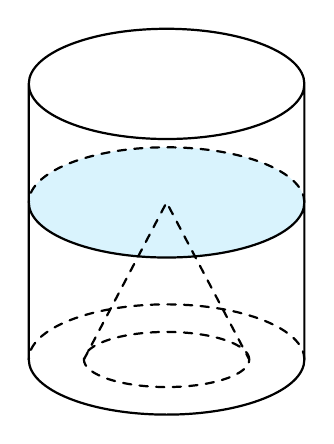
\begin{tikzpicture}[join = round, cap = round, thick, font = \footnotesize, scale = .7,>=stealth]
	\def\x{2.5}  %bán trục lớn elip 
	\def\y{1}  %bán trục bé elip 
	\def\h{5}  %chiều cao hình trụ 
	\path 
	(0:0) coordinate (O)
	+(0:\x) coordinate (A)
	+(90:\h) coordinate (O')
	(O')+(0:\x) coordinate (A')
	(O)+(180:\x) coordinate (B)
	(O')+(180:\x) coordinate (B')
	(A)+(90:2.85) coordinate(A1)
	(O)+(90:2.85) coordinate(O1)
	;
	\fill[cyan!15](O1) ellipse ({\x} and {\y});
	\draw[dashed] 
	(A) arc (0:180:{\x} and {\y})
	(A1) arc (0:180:{\x} and {\y})
	(O) ellipse ({1.5} and {.5})
	(-1.5,0)--(O1)--(1.5,0)
	;
	
	\draw 
	(A) arc (0:-180:{\x} and {\y})
	(A1) arc (0:-180:{\x} and {\y})
	(O') ellipse ({\x} and {\y})
	(A')--(A)
	(B)--(B')
	;
	%\foreach \x/\g in {O/-90,A/0,O'/90,A'/0,A1/0,O1/90}
	%\fill (\x) circle (1.5pt)
	%+(\g:3mm) node {$\x$};
\end{tikzpicture}
}
	\loigiai{
		Thể tích nước đang chứa trong hình trụ trước khi đặt khối nón vào là $26\pi r_2^2$.\\
		Thể tích nước sau khi đặt khối nón vào là $\pi r_2^2h$.\\
		Thể tích khối nón $(N)$ là $\dfrac{1}{3}\pi \cdot r_1^2h$.\\
		Ta có
		\allowdisplaybreaks
		\begin{eqnarray*}
			&&26\pi r_2^2+\dfrac{1}{3}\pi\cdot r_1^2h=\pi r_2^2h\\
			&\Leftrightarrow&26\cdot 9r_1^2+\dfrac{1}{3}r_1^2h=9r_1^2h\\
			&\Leftrightarrow&26\cdot 9+\dfrac{1}{3}h=9h\\
			&\Leftrightarrow&26\cdot 9=\dfrac{26h}{3}\\
			&\Leftrightarrow& h=27.
		\end{eqnarray*}
	}
\end{ex}
%%==========Câu 40
\begin{ex}%[2-TT-7-SGD-Hòa Bình- 2023- Lần 1]%[Nguyễn Cường-EX-6]%[2H3K3-7]
Trong KG $Oxyz$, cho mặt phẳng $(\alpha)\colon 2x-2y-z+1=0$ và hai đường thẳng $d_1\colon \heva{&x=-2+t\\&y=2+t\\&z=-t}$; $d_2\colon\heva{&x=2t'\\&y=3+t'\\&z=1}$. Gọi $\Delta$ là đường thẳng nằm trong mặt phẳng $(\alpha)$ và cắt cả hai đường thẳng $d_1$, $d_2$. Đường thẳng $\Delta$ có phương trình là
	\choice
	{\True $\dfrac{x-7}{1}=\dfrac{y-3}{-3}=\dfrac{z-9}{8}$}
	{$\dfrac{x-3}{1}=\dfrac{y-3}{-3}=\dfrac{z+1}{8}$}
	{$\dfrac{x-1}{1}=\dfrac{y+1}{-3}=\dfrac{z-5}{8}$}
	{$\dfrac{x-6}{1}=\dfrac{y-6}{3}=\dfrac{z-1}{8}$}
	\loigiai{
	Gọi $A(-2+t;2+t;-t)$ là giao điểm của $d_1$ và $(\alpha)$.\\
	Do $A\in (\alpha)$ nên $2(-2+t)-2(2+t)-(-t)+1=0\Leftrightarrow t=7$.\\
	Suy ra $A(5;9;-7)$.\\
	Tương tự gọi $B(2t';3+t';1)$ là giao điểm của $d_2$ và $(\alpha)$.\\
	Do $B\in (\alpha)$ nên $2\cdot 2t'-2(3+t')-1+1=0\Leftrightarrow t=3$.\\
	Suy ra $B(6;6;1)$.\\
	$\Delta$ nhận $\overrightarrow{AB}=(1;-3;8)$ làm véc-tơ chỉ phương.\\
	Vậy $\Delta\colon \dfrac{x-7}{1}=\dfrac{y-3}{-3}=\dfrac{z-9}{8}$ do đi qua $A(5;9;-7)$.
	}
\end{ex}
%%==========Câu 41
\begin{ex}%[2-TT-7-SGD-Hòa Bình- 2023- Lần 1]%[Nguyễn Cường-EX-6]%[2D2G4-4]
Cho $x>0$, $y>1$ thỏa mãn $\dfrac{1}{2}y^2\cdot\log_2\left(\dfrac{xy-x}{2y}\right)=-2(y-1)^2+\dfrac{8y^2}{x^2}$. Giá trị nhỏ nhất của $P=\sqrt[4]{\mathrm{e}^{\tfrac{x^2}{1+2y}}}\cdot \mathrm{e}^{\tfrac{y^2}{x+1}}$ có dạng $\mathrm{e}^{\tfrac{m}{n}}$ (trong đó $m$, $n$ là các số nguyên dương, $\dfrac{m}{n}$ là phân số tối giản). Giá trị của $m+n$ bằng
	\choice
	{\True $12$}
	{$21$}
	{$22$}
	{\True $13$}
	\loigiai
	{
		Ta có
		\allowdisplaybreaks
		\begin{eqnarray*}
		&&\dfrac{1}{2}y^2\cdot\log_2\left(\dfrac{xy-x}{2y}\right)=-2(y-1)^2+\dfrac{8y^2}{x^2}\\
		&\Leftrightarrow&\dfrac{1}{2}y^2\cdot\log_2\left(\dfrac{x(y-1)}{2y}\right)=-2(y-1)^2+\dfrac{8y^2}{x^2}\\
		&\Leftrightarrow&\log_2\left(\dfrac{x(y-1)}{2y}\right)=\dfrac{-4(y-1)^2}{y^2}+\dfrac{16}{x^2}\\
		&\Leftrightarrow&\log_2x+\log_2\dfrac{y-1}{2y}=-16\cdot \dfrac{(y-1)^2}{4y^2}+\dfrac{16}{x^2}\\
		&\Leftrightarrow&\log_2x+\log_2\dfrac{y-1}{2y}=-16\cdot \left(\dfrac{y-1}{2y}\right)^2+\dfrac{16}{x^2}\\
		&\Leftrightarrow&\log_2\dfrac{y-1}{2y}+16\cdot \left(\dfrac{y-1}{2y}\right)^2=\log_2\dfrac{1}{x}+\dfrac{16}{x^2}.
		\end{eqnarray*}
	Xét hàm số $f(t)=\log_2t+16t^2$ trên $(0;+\infty)$.\\
	Do $f'(t)=\dfrac{1}{t\ln 2}+32t>0$ với mọi $t>0$ nên hàm số $f(t)$ đồng biến trên $(0;+\infty)$.\\
	Mặt khác $f\left(\dfrac{y-1}{2y}\right)=f\left(\dfrac{1}{x}\right)$ nên $\dfrac{y-1}{2y}=\dfrac{1}{x}$.\\
	Khi đó, $P=\sqrt[4]{\mathrm{e}^{\tfrac{x^2}{1+2y}}}\cdot \mathrm{e}^{\tfrac{y^2}{x+1}}=\mathrm{e}^{\tfrac{x^2}{4(1+2y)}}\cdot \mathrm{e}^{\tfrac{y^2}{x+1}}=\mathrm{e}^{\tfrac{x^2}{4(1+2y)}+\tfrac{y^2}{x+1}}$.\\
	Với $x=\dfrac{2y}{y-1}$, ta xét hàm số $f(y)=\dfrac{y^2}{(y-1)^2(1+2y)}+\dfrac{y^2(y-1)}{3y-1}$ với $y>1$.\\
	Ta có $f'(y)=2y(y-2)\cdot\dfrac{12y^6-12y^5+7y^4+9y^3-2y^2-3y+1}{(y-1)^3(2y+1)^2(3y-1)^2}$.\\
	Hàm số đạt cực trị tại $y=2$ và giá trị nhỏ nhất của hàm số $f(y)=f(2)=\dfrac{8}{5}$.\\
	Vậy $m+n=13$.\\
	\textbf{Nhận xét:} Có thể dùng chắc năng Table của máy tính Casio để dò tìm cực trị của hàm số này vì bài toán đưa ra hàm số phức tạp và tính toán đạo hàm đưa đến bậc cao.
	}
\end{ex}
%%==========Câu 42
\begin{ex}%[2-TT-7-SGD-Hòa Bình- 2023- Lần 1]%[Nguyễn Cường-EX-6]%[2D1K5-4]
	\immini{
	Cho hàm số bậc bốn $y=f(x)$ có đồ thị là đường cong như hình bên. Đặt $g(x)=f(f(x)-1)$, gọi $S$ là tập nghiệm của phương trình $g(x)=0$. Số phần tử của tập $S$ là 
	\choice
	{$6$}
	{$8$}
	{\True $7$}
	{$9$}
}
{
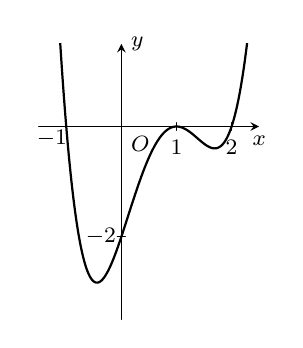
\begin{tikzpicture}[scale=.7,>=stealth, font=\footnotesize, line join=round, line cap=round]
	%Hệ trục Oxy và hàm số cần vẽ
	\def\xmin{-1.5}     \def\xmax{2.5}
	\def\ymin{-3.5}       \def\ymax{1.5}
	%Vẽ hệ trục
	\draw[->] (\xmin,0)--(0,0) node[below right]{$O$}--(\xmax,0) node[below]{$x$};
	\draw[->] (0,\ymin)--(0,\ymax) node[right]{$y$};
	%Vẽ hàm số
	\begin{scope}
		\clip (\xmin,\ymin) rectangle (\xmax,\ymax);
		\draw[smooth, thick] plot[domain = \xmin:\xmax, samples = 200, variable=\x]({\x},{((\x)+1)*((\x)-1)^2*((\x)-2)});
	\end{scope}
	%Vẽ các điểm trên trục Ox
	\foreach \x/\g in {-1/-150,1/-90,2/-90}
	\draw[thin] (\x,2pt)--(\x,-2pt) + (\g:3mm) node {$\x$};
	%Vẽ các điểm trên trục Oy
	\foreach \y/\g in {-2/180}
	\draw[thin] (2pt,\y)--(-2pt,\y) + (\g:3mm) node {$\y$};
\end{tikzpicture}
}
	\loigiai
	{
		Ta có $g(x)=0\Leftrightarrow \hoac{&f(x)-1=-1\\&f(x)-1=1\\&f(x)-1=2}\Leftrightarrow\hoac{&f(x)=0\\&f(x)=2\\&f(x)=3.}$\\
		Dựa vào đồ thị hàm số 
		\begin{itemize}
			\item Phương trình $f(x)=0$ có $3$ nghiệm.
			\item Phương trình $f(x)=2$ có $2$ nghiệm.
			\item Phương trình $f(x)=3$ có $2$ nghiệm.
		\end{itemize}
	Vậy phương trình $g(x)=0$ có $7$ nghiệm phân biệt.
	}
\end{ex}
%%==========Câu 43
\begin{ex}%[2-TT-7-SGD-Hòa Bình- 2023- Lần 1]%[Nguyễn Cường-EX-6]%[2H1K3-3]
	Cho hình chóp $S.ABCD$ có đáy là hình chữ nhật $ABCD$ cạnh $AB=2a$, $BC=a$, $SA$ vuông góc với mặt đáy và cạnh $SC$ tạo với mặt phẳng $(ABCD)$ một góc $\alpha$ có $\tan\alpha=\dfrac{\sqrt{5}}{5}$. Gọi $E$, $F$ lần lượt là các điểm nằm trên cạnh $SB$, $SD$ sao cho $SB=2SE$, $SD=3SF$. Thể tích $V$ của khối tứ diện $AEFC$ là
	\choice
	{$V=\dfrac{a^3}{3}$}
	{$V=\dfrac{a^3\sqrt{3}}{6}$}
	{\True $V=\dfrac{a^3}{6}$}
	{$V=\dfrac{a^3}{2}$}
	\loigiai{
		\immini{
		Đường chéo $AC=\sqrt{AB^2+BC^2}=a\sqrt{5}$.\\
		Góc giữa $SC$ và đáy $(ABCD)$ là $\widehat{SCA}$.\\
		Do $\tan\widehat{SCA}=\dfrac{SA}{AC}\Rightarrow SA=AC\cdot \tan \widehat{SCA}=a\sqrt{5}\cdot \dfrac{\sqrt{5}}{5}=a$.\\
		Thể tích khối chóp $V=V_{S.ABCD}=\dfrac{1}{3}\cdot SA\cdot S_{ABCD}=\dfrac{1}{3}\cdot a\cdot 2a\cdot a=\dfrac{2a^3}{3}$.
		\begin{itemize}
			\item $V_1=V_{S.AEF}=\dfrac{SA}{SA}\cdot \dfrac{SE}{SB}\cdot \dfrac{SF}{SD}\cdot V_{S.ABD}=1\cdot \dfrac{1}{2}\cdot \dfrac{1}{3}\cdot\dfrac{V}{2}=\dfrac{V}{12}$.
			\item $V_2=V_{F.ACD}=\dfrac{2}{3}\cdot V_{S.ACD}=\dfrac{2}{3}\cdot \dfrac{V}{2}=\dfrac{V}{3}$.
			\item $V_3=V_{E.ABC}=\dfrac{1}{2}\cdot V_{S.ABC}=\dfrac{1}{2}\cdot \dfrac{V}{2}=\dfrac{V}{4}$.
			\item $V_4=V_{S.CEF}=\dfrac{SC}{SC}\cdot \dfrac{SE}{SB}\cdot \dfrac{SF}{SD}\cdot V_{S.CBD}=1\cdot \dfrac{1}{2}\cdot \dfrac{1}{3}\cdot\dfrac{V}{2}=\dfrac{V}{12}$.
		\end{itemize}
	Vậy $V_{A.EFC}=V-\left(\dfrac{V}{12}+\dfrac{V}{3}+\dfrac{V}{4}+\dfrac{V}{12}\right)=\dfrac{V}{4}=\dfrac{a^3}{6}$.
		}
		{
			\begin{tikzpicture}[font=\footnotesize,line join=round, line cap=round, >=stealth,scale=0.8]
					\path 
					(0:0) coordinate (A)
					+(0:5) coordinate (B)
					+(-150:2.5) coordinate (D)
					+(90:4) coordinate (S)
					($(B)+(D)-(A)$) coordinate (C)
					($(S)!.5!(B)$) coordinate (E)
					($(S)!1/3!(D)$) coordinate (F)
					;
					\draw[dashed] 
					(A)--(B) (A)--(D) (C)--(A)--(S)
					(A)--(E)--(F)--cycle
					;
					\draw 
					(D)--(C)--(B)
					(S)--(B) (S)--(C)--(E) (C)--(F) (S)--(D)
					\foreach \x/\y/\z in {S/A/B,S/A/D}{
						pic[draw, angle radius = 6pt]{right angle = \x--\y--\z}
					}
					;
					\foreach \x/\g in {A/135,B/0,C/-45,D/-135,S/90,E/45,F/120}
					\fill (\x) circle (1.5pt)
					+(\g:3.5mm) node {$\x$};
		\end{tikzpicture}}
	}
\end{ex}
%%==========Câu 44
\begin{ex}%[2-TT-7-SGD-Hòa Bình- 2023- Lần 1]%[Nguyễn Cường-EX-6]%[2D3K3-1]
	Cho hai hàm số $f(x)=ax^4+bx^3+cx^2+3x$ và $g(x)=mx^3+nx^2-x$ với $a$, $b$, $c$, $m$, $n\in\mathbb{R}$. Biết hàm số $y=f(x)-g(x)$ có ba điểm cực trị là $-1$; $1$ và $2$. Diện tích hình phẳng giới hạn bởi hai đường $y=f'(x)$ và $y=g'(x)$ bằng
	\choice
	{$\dfrac{5}{6}$}
	{$\dfrac{9}{2}$}
	{\True $\dfrac{37}{6}$}
	{$\dfrac{16}{3}$}
	\loigiai
	{
	Hàm số $y=f(x)-g(x)$ có đạo hàm $$y'=f'(x)-g'(x)=4ax^3+3bx^2+2cx+3-3mx^2-2nx+1=4ax^3+(3b-3m)x^2+(2c-2n)x+4.$$
	Do $y=f(x)-g(x)$ có ba điểm cực trị là $-1$; $1$ và $2$ nên $y'=4a(x+1)(x-1)(x-2)=4a(x^3-2x^2-x+2)$.\\
	Khi đó $\heva{&3b-3m=-8a\\&2c-2n=-4a\\&4=8a}\Leftrightarrow\heva{&3b-3m=-4\\&2c-2n=-2\\&a=\dfrac{1}{2}.}$\\
	Suy ra $f'(x)-g'(x)=2x^3-4x^2-2x+4$.\\
	Xét phương trình $f'(x)=g'(x)\Leftrightarrow 2x^3-4x^2-2x+4=0\Leftrightarrow\hoac{&x=-1\\&x=1\\&x=2.}$\\ 
	Do đó, diện tích cần tìm là $S=\displaystyle\int\limits_{-1}^2\left|f'(x)-g'(x)\right|\mathrm{\,d}x=\displaystyle\int\limits_{-1}^2\left|2x^3-4x^2-2x+4\right|\mathrm{\,d}x=\dfrac{37}{6}$.
	}
\end{ex}
%%==========Câu 45
\begin{ex}%[2-TT-7-SGD-Hòa Bình- 2023- Lần 1]%[Nguyễn Cường-EX-6]%[2D4G2-4]
Cho các số phức $z_1$; $z_2$; $z_3$ thỏa mãn $|z_1|=|z_2|=3$; $z_2+z_3=0$ và $z_1z_2z_3=9(z_1+z_2)$. Gọi $A$, $B$, $C$ lần lượt là điểm biểu diễn của số phức $z_1$; $z_2$; $z_3$. Diện tích tam giác $ABC$ bằng
	\choice
	{\True $\dfrac{9\sqrt{3}}{2}$}
	{$\dfrac{9\sqrt{3}}{4}$}
	{$9\sqrt{3}$}
	{$18$}
	\loigiai
	{
	\immini
	{
Tập hợp các điểm biểu diễn của $z_1$; $z_2$ là đường tròn tâm $O(0;0)$ và bán kính $R=3$.\\
Do $z_2+z_3=0$ nên điểm $B$ và $C$ đối xứng nhau qua gốc tọa độ $O$, đồng thời $BC$ là đường kính của đường tròn.\\
Suy ra $\triangle ABC$ vuông tại $A$.\\
Ta có $BC=|z_2-z_3|=|2z_2|=6$.\\
Mà $z_1z_2z_3=9(z_1+z_2)\Leftrightarrow |z_1z_2z_3|=9|z_1+z_2|\Rightarrow |z_1+z_2|=3$.\\
Ta lại có $|z_1-z_2|^2+|z_1+z_2|^2=2\left(|z_1|^2+|z_2|^2\right)\Leftrightarrow |z_1-z_2|^2=27$ hay $AB=3\sqrt{3}$.\\
Khi đó, $AC=\sqrt{BC^2-AB^2}=3$.\\
Vậy $S_{ABC}=\dfrac{1}{2}\cdot AB\cdot AC=\dfrac{9\sqrt{3}}{2}$.
}
{

}
	}
\end{ex}
%%==========Câu 46
\begin{ex}%[2-TT-7-SGD-Hòa Bình- 2023- Lần 1]%[Nguyễn Cường-EX-6]%[2D2G6-5]
Cho bất phương trình $\log_5(x^2+1)>\log_5(x^2+6x+m)-1$. Có bao nhiêu giá trị nguyên của tham số $m$ để bất phương trình trên có tập nghiệm chứa khoảng $(2;3)$?
		\choice
		{$27$}
		{$24$}
		{\True $26$}
		{$25$}
	\loigiai
	{
Ta có $\log_5(x^2+1)>\log_5(x^2+6x+m)-1\Leftrightarrow \heva{&x^2+6x+m>0\\&x^2+1>\dfrac{x^2+6x+m}{5}}\Leftrightarrow\heva{&m>-x^2-6x\\&m<4x^2-6x+5.}$\\
Xét hàm số $f(x)=-x^2-6x$ trên $(2;3)$.\\
Ta có $f'(x)=-2x-6<0$ với mọi $x\in (2;3)$.\\
Suy ra trên $(2;3)$ ta có $m>-x^2-6x\Leftrightarrow m\ge f(2)=-16$.\\
Xét hàm số $h(x)=4x^2-6x+5$ trên $(2;3)$.\\
Có $h'(x)=8x-6>0$ với mọi $x\in (2;3)$.\\
Suy ra trên $(2;3)$ ta có $m<4x^2-6x+5\Leftrightarrow m\le h(2)=9$.\\
Vậy $-16\le m\le 9$, mà $m\in \mathbb{Z}$ nên có $26$ giá trị nguyên thỏa mãn yêu cầu bài toán.
}
\end{ex}
%%==========Câu 47
\begin{ex}%[2-TT-7-SGD-Hòa Bình- 2023- Lần 1]%[Nguyễn Cường-EX-6]%[2D4G4-3]
Cho phương trình $z^2+az+b=0$ với $a$, $b\in\mathbb{R}$ có hai nghiệm $z_1$, $z_2$ không là số thực; thỏa mãn hệ thức $i|z_1|=z_2+i-3$. Giá trị của $2a+b$ bằng
		\choice
		{$10$}
		{$37$}
		{\True $13$}
		{$25$}
	\loigiai{
		Do $z_1$; $z_2$ không là số thực nên hai nghiệm này là liên hợp của nhau và $|z_1|=|z_2|$.\\
		Ta có 
		\allowdisplaybreaks
		\begin{eqnarray*}
			i|z_1|=z_2+i-3&\Leftrightarrow&i|z_2|=z_2+i-3\\
			&\Leftrightarrow&3+i\left(|z_2|-1\right)=z_2\\
			&\Leftrightarrow&\sqrt{9+\left(|z_2|-1\right)^2}=|z_2|\\
			&\Leftrightarrow&9+|z_2|^2-2|z_2|+1=|z_2|^2\\
			&\Leftrightarrow& |z_2|=5.
		\end{eqnarray*}
	Suy ra, $z_2=3+i\left(|z_2|-1\right)=3+4i$ và $z_1=3-4i$.\\
	Ta có $z_1+z_2=-a=6\Leftrightarrow a=-6$ và $z_1z_2=b=25$.\\
	Vậy $2a+b=-12+25=13$.
	}
\end{ex}
%%==========Câu 48
\begin{ex}%[2-TT-7-SGD-Hòa Bình- 2023- Lần 1]%[Nguyễn Cường-EX-6]%[2D1G2-6]
	\immini{Cho hàm số $y=f(x)$ có đạo hàm liên tục trên $\mathbb{R}$, đồ thị của hàm số $y=f'(x)$ có đúng bốn điểm chung với trục hoành như hình vẽ bên. Có bao nhiêu giá trị nguyên của tham số $m$ để hàm số $y=f\left(|x|^3-3|x|+m+2023\right)+2023m$ có $11$ điểm cực trị.
		\choice
		{$0$}
		{$2$}
		{$5$}
		{\True $1$}}
	{
		\begin{tikzpicture}[>=stealth,line join=round,line cap=round,font=\footnotesize,scale=1.0]
			\def \xmin{-2}
			\def \xmax{5}
			\def \ymin{-1}
			\def \ymax{3.5}
			\draw[->] (\xmin,0)--(\xmax,0) node[below] {$x$};
			\draw[->] (0,\ymin)--(0,\ymax) node[left] {$y$};
			\fill (0,0) node[shift={(135:.25)}] {$O$} circle(1pt);
			\begin{scope}
				\clip (\xmin,\ymin) rectangle (\xmax,\ymax);
				\draw (-1.2,-1) ..controls +(90:0.3) and +(180:0.4).. (0,2.5)..controls +(0:0.4) and +(180:0.5)..(1.4,-0.6) ..controls +(0:0.4) and +(180:0.5).. (2.8,0.8) ..controls +(0:0.4) and +(180:0.4).. (4,0) ..controls +(0:0.5) and +(-90:0.2).. (5.5,\ymax);
			\end{scope}
			\foreach \x in{-1, 1, 2, 4} \fill (\x,0) node[shift={(-90:0.35)}]{$\x$} circle(1pt);
	\end{tikzpicture}}
	\loigiai{
		Vì hàm số $y=f\left(|x|^3-3|x|+m+2023\right)+2023m$ là hàm số chẵn nên hàm số có $11$ điểm cực trị khi và chỉ khi hàm số $g(x)=f\left(x^3-3x+m+2023\right)$ có đúng $5$ điểm cực trị trên $(0; +\infty)$, tức là phương trình $g'(x)=0$ có đúng $5$ nghiệm bội lẻ dương.\\
		Ta có $g'(x)=\left(3x^2-3\right)f'\left(x^3-3x+m+2023\right)$ nên
		\[g'(x)=0 \Leftrightarrow \hoac{&x=1 \\ &x=-1 \quad \text{(loại)} \\&f'\left(x^3-3x+m+2023\right)=0.}\]
		Từ đồ thị của hàm số $y=f'(x)$, ta có
		\[f'\left(x^3-3x+m+2023\right)=0 \Leftrightarrow \hoac{&x^3-3x+2023=-m+4 \\&x^3-3x+2023=-m+2 \\&x^3-3x+2023=-m+1 \\&x^3-3x+2023=-m-1.}\]
		Xét hàm số $h(x)=x^3-3x+2023$ trên $(0;+\infty)$, ta có $h'(x)=3x^2-3$ và bảng biến thiên
		\begin{center}
			
\begin{tikzpicture}[>=stealth]
				\tkzTabInit[nocadre=false,lgt=1.2,espcl=2,deltacl=0.5]{$x$/.7 ,$h'(x)$/.7,$h(x)$/2}
				{$-1$ , $0$ , $1$ , $+\infty$}
				\tkzTabLine{ 0, - , t , - , $0$ , + , }
				\tkzTabVar{+/$2025$ , R , -/$2021$ , +/$+\infty$}
				\tkzTabIma{1}{3}{2}{$2023$}
			\end{tikzpicture}
		\end{center}
		Vì $x=4$ là nghiệm bội chẵn của phương trình $f'(x)=0$ nên từ bảng biến thiên này, với $m$ nguyên, ta thấy rằng $g'(x)=0$ có đúng $5$ nghiệm bội lẻ dương khi vào chỉ khi $-m-1=2022 \Leftrightarrow  m=-2023$.\\
		Vậy, có đúng một giá trị $m=-2023$ thỏa bài toán.
	}
\end{ex}
%%==========Câu 49
\begin{ex}%[2-TT-7-SGD-Hòa Bình- 2023- Lần 1]%[Nguyễn Cường-EX-6]%[2H3G1-4]
	Trong KG $Oxyz$, cho mặt cầu $(S)\colon (x-1)^2+(y-2)^2+(z+1)^2=9$ và điểm $M(4;2;3)$. Một đường thẳng bất kỳ qua $M$ cắt $(S)$ tại $A$, $B$. Khi đó giá trị nhỏ nhất của $MA^2+4MB^2$ bằng
	\choice
	{\True $64$}
	{$32$}
	{$16$}
	{$8$}
	\loigiai{
	Ta có $MA^2+4MB^2\ge 2\sqrt{MA^2\cdot 4MB^2}=4MA\cdot MB$.\\
	Mặt cầu $(S)$ có tâm $I(1;2;-1)$ và bán kính $R=3$.\\
	Theo phương tích của $M$ và mặt cầu $(S)$ ta có $MA\cdot MB=MI^2-R^2=16$.\\
	Vậy giá trị nhỏ nhất của $MA^2+4MB^2$ là $4MA\cdot MB=4\cdot 16=64$.
	}
\end{ex}
%%==========Câu 50
\begin{ex}%[2-TT-7-SGD-Hòa Bình- 2023- Lần 1]%[Nguyễn Cường-EX-6]%[2D3G2-4]
	Cho hàm số $f(x)$ có đạo hàm liên tục trên $[0;1]$ thỏa mãn $f(1)=4$; $f(0)=1$ và $\displaystyle\int\limits_0^1\left[f'(x)\right]^2\mathrm{\,d}x=9$. Giá trị của tích phân $\displaystyle\int\limits_0^1xf^2(x)\mathrm{\,d}x$ bằng
	\choice
	{$\dfrac{1}{4}$}
	{$9$}
	{$\dfrac{1}{6}$}
	{\True $\dfrac{19}{4}$}
	\loigiai
	{
	Do $f(x)$ có đạo hàm liên tục trên $[0;1]$ nên $\displaystyle\int\limits_0^1f'(x)\mathrm{\,d}x=f(1)-f(0)=3$.\\
Ta có $\displaystyle\int\limits_0^1\left[f'^2(x)-6f'(x)+9\right]\mathrm{\,d}x=\displaystyle\int\limits_0^1f'^2(x)\mathrm{\,d}x-6\displaystyle\int\limits_0^1f'(x)\mathrm{\,d}x+\displaystyle\int\limits_0^19\mathrm{\,d}x=9-18+9=0$.\\
Suy ra $\displaystyle\int\limits_0^1\left[f'(x)-3\right]^2\mathrm{\,d}x=0\Rightarrow f'(x)-3=0$.\\
Do đó, $f(x)=3x+C$.\\
Mà $f(0)=1$ nên $C=1$, suy ra $f(x)=3x+1$.\\
Vậy $\displaystyle\int\limits_0^1xf^2(x)\mathrm{\,d}x=\displaystyle\int\limits_0^1x(3x+1)^2\mathrm{\,d}x=\dfrac{19}{4}$.
}
\end{ex}
\Closesolutionfile{ans}
\begin{indapan}{10}
	{ans/ans-2-TT-7-SGD-HoaBinh-23-L1}
\end{indapan}


